\documentclass[a4paper, 11pt]{article}
\usepackage[a4paper, left=1in, right=1in, top=1in, bottom=1in]{geometry}
\usepackage[dvipsnames]{xcolor}
\usepackage{graphicx} % Required for inserting images
\usepackage{amsfonts}
\usepackage{amssymb}
\usepackage{amsmath}
\usepackage{tikz,lipsum,lmodern}
\usepackage[most]{tcolorbox}
\usepackage{pgfplots}
\usepackage{tabularx}
\usepackage{stmaryrd}
\usepackage{tikz} 
\usepackage{imakeidx}
\usepackage{blindtext}
\usepackage{hyperref}
\usepackage[rightcaption]{sidecap}
\usepackage{wrapfig}
\usepackage{cancel}
\usepackage{titlesec}
\usepackage{enumitem}
\usepackage{float}
\usepackage{tabularx}
\usepackage{adjustbox}
\usepackage{multicol}
\usepackage{listings}
\setlist{nolistsep} % Rimuove lo spazio extra tra gli elementi della lista

\definecolor{comment}{rgb}{0.5, 0.5, 0.5}
\definecolor{string}{rgb}{0.3, 0.6, 0.3}
\definecolor{keyword}{rgb}{0.7, 0, 0.4}
\definecolor{identifier}{rgb}{0.2, 0.2, 1}
\definecolor{background}{rgb}{0.99, 0.99, 0.99}

\lstdefinestyle{customcpp}{
    language=C++,
    basicstyle=\ttfamily\footnotesize,
    backgroundcolor=\color{background},
    keywordstyle=\color{keyword},
    identifierstyle=\color{identifier},
    commentstyle=\color{comment}\itshape,
    stringstyle=\color{string},
    numbers=left,
    numberstyle=\tiny\color{gray},
    stepnumber=1,
    numbersep=10pt,
    tabsize=4,
    showspaces=false,
    showstringspaces=false,
    breaklines=true,
    breakatwhitespace=true,
    escapeinside={\%*}{*)},
    frame=single,
    rulecolor=\color{black},
    captionpos=b,
    morekeywords={override, nullptr},
}
\titleformat{\chapter}[display]
  {\normalfont\Large\bfseries} % Stile del titolo
  {\chaptername\ \thechapter}{10pt}{\Large}

\titlespacing*{\chapter}{0pt}{-20pt}{20pt}

\newenvironment{myindentpar}[1]%
  {\begin{list}{}%
          {\setlength{\leftmargin}{#1}}%
          \item[]%
  }
  {\end{list}}

\hypersetup{
    colorlinks=true,
    linkcolor=black,
    filecolor=magenta,      
    urlcolor=blue,
    pdftitle={Relazione_Centro-Controllo-Droni},
    pdfpagemode=FullScreen,
}

\setlength{\parindent}{0pt}
\setlength{\parskip}{5pt}


\makeindex[columns=3, title=Alphabetical Index, intoc]
\hypersetup{
    colorlinks=true,
    linkcolor=blue!50!green,
    filecolor=magenta,      
    urlcolor=cyan,
    pdftitle={Overleaf Example},
    pdfpagemode=FullScreen,
    }

\newcommand\scalemath[2]{\scalebox{#1}{\mbox{\ensuremath{\displaystyle #2}}}}
\definecolor{bananamania}{rgb}{0.98, 0.91, 0.71}
\definecolor{amaranth}{rgb}{0.9, 0.17, 0.31}
\definecolor{amethyst}{rgb}{0.6, 0.4, 0.8}
\definecolor{darktangerine}{rgb}{1.0, 0.66, 0.07}
\definecolor{cerise}{rgb}{0.87, 0.19, 0.39}
\definecolor{babyblue}{rgb}{0.54, 0.81, 0.94}


\title{Relazione su \\
Controllo formazione droni}
\author{A. Bettoni (1998044),\\ A. Coppola (2003964),\\S. Di Cesare (1938649)}
\date{\today}

\begin{document}
\maketitle
\newpage
\tableofcontents
\newpage
\section{Descrizione Generale}
\paragraph*{Problema:}
Si vuole progettare un sistema di controllo di n droni che sorvegli una data area rettangolare.
Il sistema deve garantire che, con i droni forniti, ogni punto dell'area venga sorvegliato il più frequentemente possibile.

I droni partiranno dalla torre di controllo che si trova al centro dell'area da sorvegliare.
Ogni drone ha un'autonomia limitata (misurata in minuti in volo) e una velocità massima. 
La torre dovrà gestire gli spostamenti di ogni drone facendo in modo che tornino alla torre prima che la batteria sia del tutto esaurita. 
Quando i droni si trovano nella torre di controllo sono considerati in carica e il tempo di ricarica può variare da drone a drone.
\paragraph*{Idea di soluzione:}
Abbiamo scelto di modellare il problema con un sistema che agisce sulla torre di controllo e ricarica che a sua volta controlla i droni.
Dunque la torre invia ad ogni drone le coordinate del punto sull'area da raggiunge secondo un sistema di volo a "tappe".
Una volta che il drone arriva alla posizione ricevuta lo comunica alla torre che risponde con la posizione successiva, delineando così un percorso.
Quando il drone è scarico lo comunica alla torre e si direziona alla torre di controllo, per essere ricaricato.

Sta al sistema quindi il compito di calcolare, mentre i droni sono in volo, il percorso migliore per far sì che ogni punto dell'area venga sorvegliato 
il più frequentemente possibile, tenendo conto dei punti visitati, dei droni in volo, e dei punti che visitano prima di scaricarsi.
\begin{figure}[h]
    \centering
    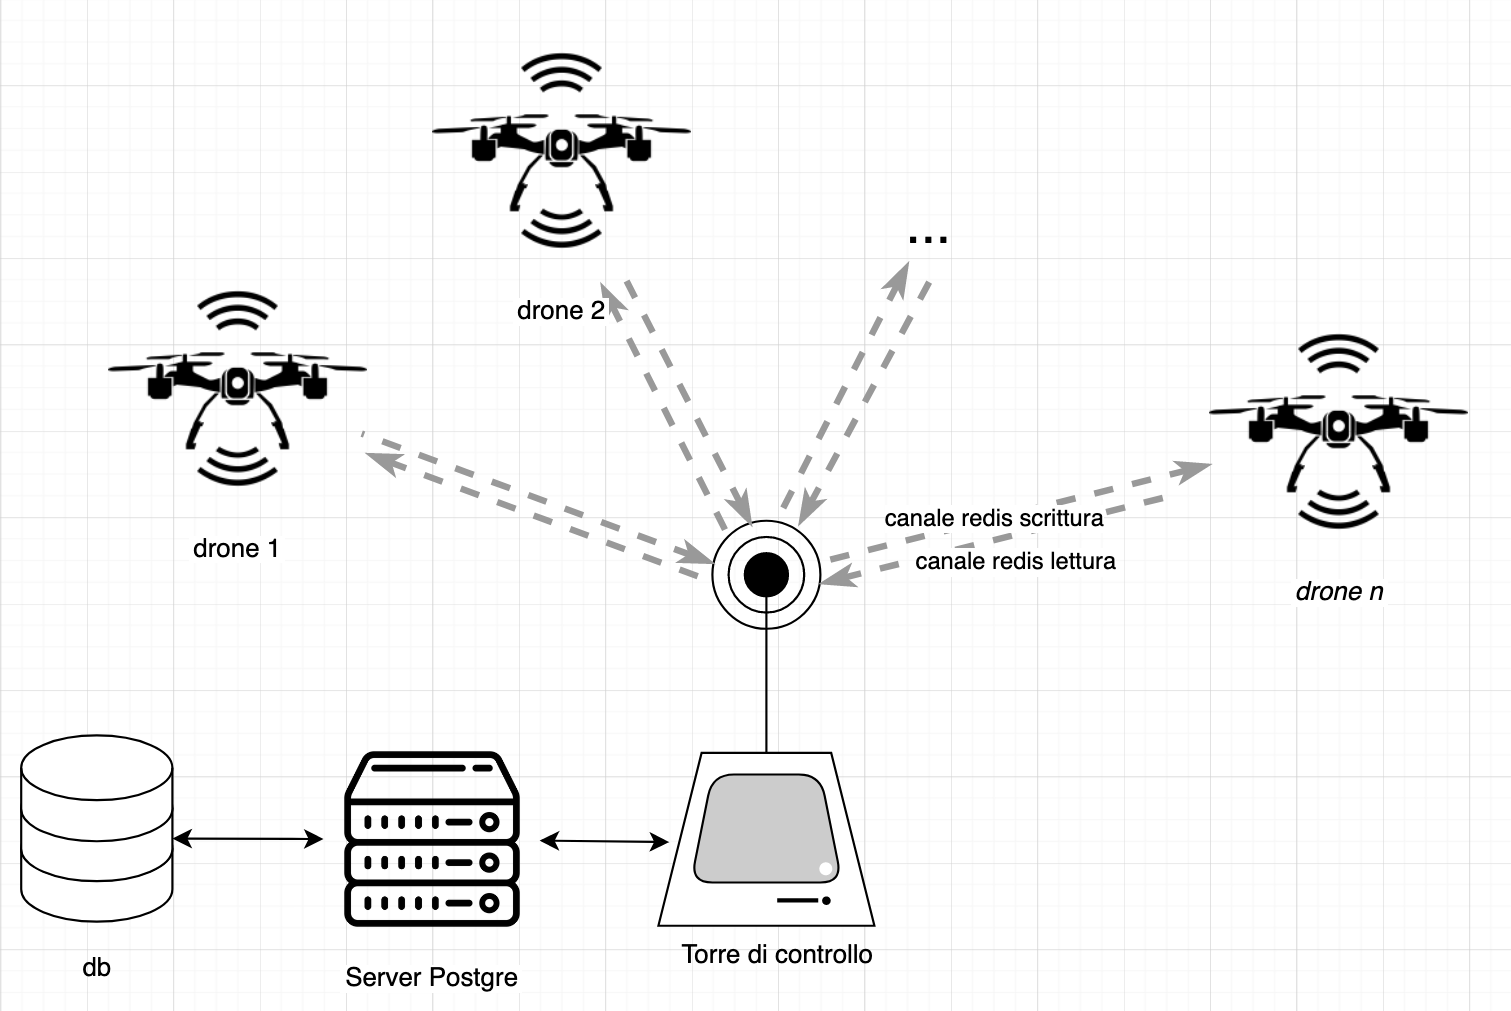
\includegraphics[height = 7.2 cm]{image/Architettura.png}\\
    \caption{Architettura fisica del sistema}
\end{figure}
\newpage

\section{Analisi del software}
\subsection{Requisiti utente}
Per funzionare, il sistema ha bisogno dei seguenti requisiti:
\begin{itemize}
    \item dimensione dell'area\\
    dato che l'area verrà divisa in blocchi, per ogni blocco è di interesse:
    \begin{itemize}
        \item limite alto superiore
        \item limite basso inferiore
        \item punto di partenza (o ultimo punto visitato)
        \item Ogni punto dell'area è identificato dalla sua posizione in una matrice di punti e di quei punti ci interessa solo:
        \begin{itemize}
            \item il tempo trascorso dall'ultima visita.
        \end{itemize}
    \end{itemize}
    \item numero di droni\\
    per ogni drone è di interesse:
    \begin{itemize}
        \item id: identificativo univoco seriale
        \item Stato : tra i stati precedentemente elencati
        \item posizione 
        \item carica residua (in minuti)
        \item carica massima (in minuti)
        \item tempo di ricarica 
        \item last\_update : tempo trascorso dall'ultimo update
    \end{itemize}
    
\end{itemize}
\newpage
\subsection{Requisiti di sistema}
Il sistema deve rispettare i seguenti requisiti:
\begin{enumerate}
    \item Area:
    \begin{enumerate}[label=1.\arabic*]
        \item I blocchi sono tutti tra loro disgiunti (non esiste un punto dell'area che si trova in più di un blocco)
        \item L'unione dei blocchi copre tutti e solo i punti dell'area (un punto appartiene all'area se e solo se esiste un blocco che lo contiene)
        \item Un blocco può essere assegnato al più ad un drone 
    \end{enumerate}
    \item Drone:
    \begin{enumerate}[label=1.\arabic*]
        \item Un drone a cui è stato assegnato un blocco può trovarsi al di fuori di esso se e solo se:
        \begin{enumerate}
            \item il drone è partito dalla torre e si sta posizionando verso il punto di partenza del blocco
            \item il drone è scarico e sta tornando alla torre
            \item il drone ha visitato tutto il blocco e si sta posizionando verso il punto di partenza di un'altro blocco
        \end{enumerate}
        \item Un drone può volare verso un punto diverso da quello della torre se e solo se il suo tempo di volo residuo è maggiore del tempo che serve al drone per andare dalla sua posizione attuale a quella della torre
    \end{enumerate}
    \item Torre:
    \begin{enumerate}[label=1.\arabic*]
        \item La torre non può terminare il suo processo se esiste un drone connesso che non è tornato nella torre di controllo.
        \item Tutti i punti che la torre invia ad un drone devono trovarsi all'interno dell'area assegnata al drone
    \end{enumerate}
    \item Requisiti non-funzionali:
    \begin{enumerate}[label=1.\arabic*]
        \item ogni punto dell'area deve essere visitato il più frequentemente possibile
        \item Il tempo di risposta della torre per ogni drone deve essere ragionevolmente basso per fare in modo che i droni rimangano fermi sul posto il meno possibile
    \end{enumerate} 
\end{enumerate}
\newpage
\subsection{Diagrams}
\begin{figure}[htbp]
    \centering
    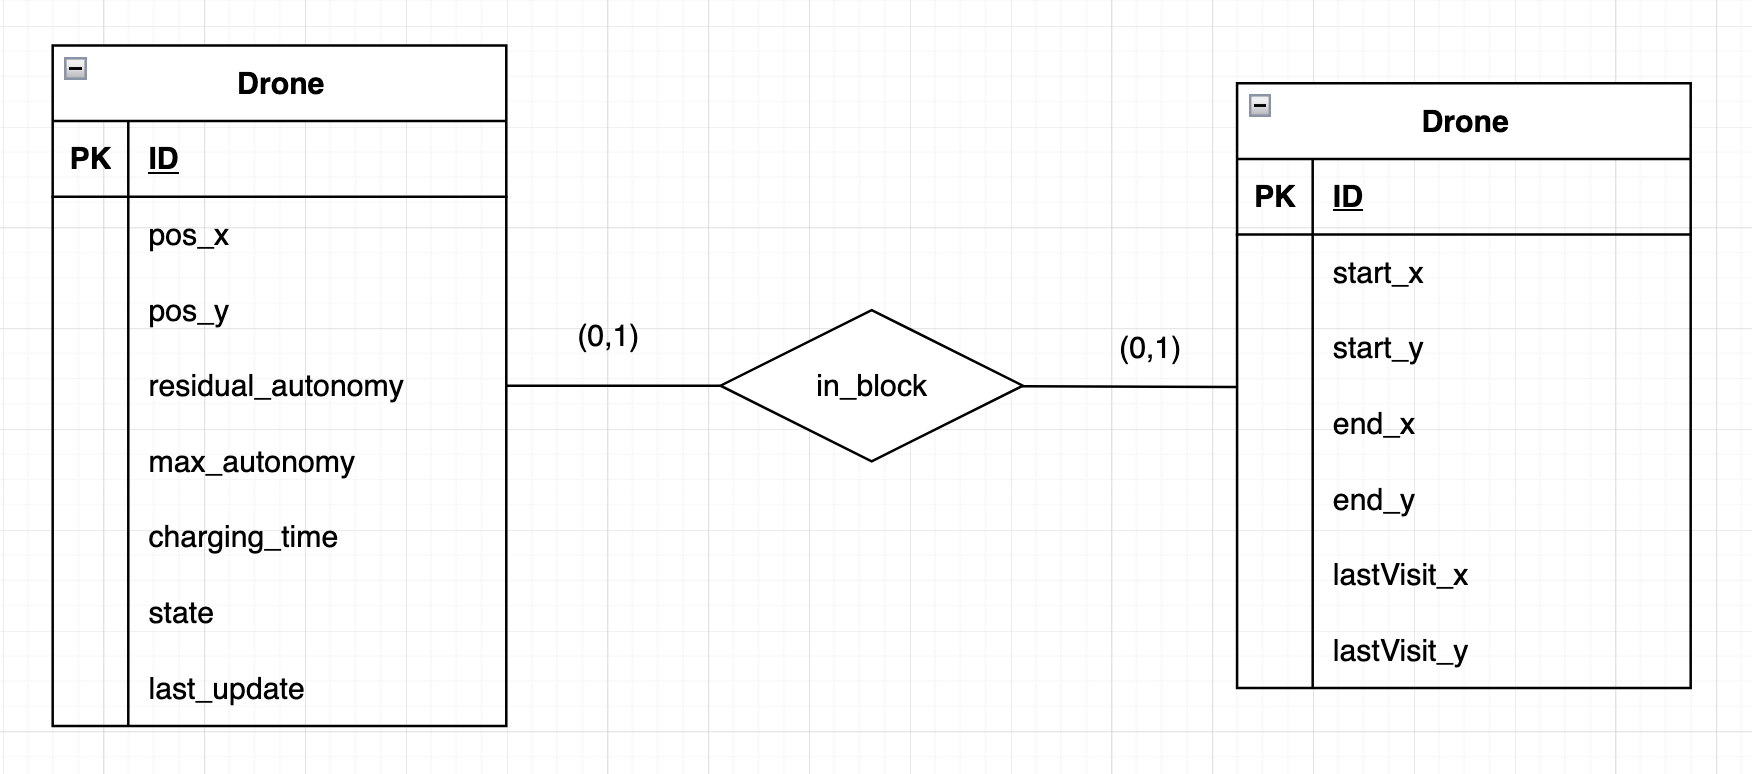
\includegraphics[height = 4 cm]{image/ER1.png}%
    \qquad\qquad
    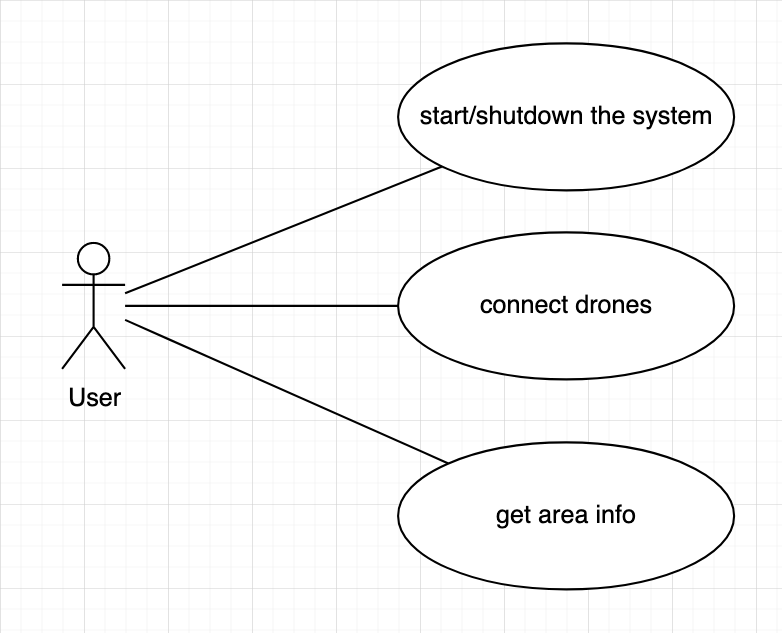
\includegraphics[height = 4 cm]{image/UML1.png}
    \caption{schema ER e UML}
\end{figure}


\subsection{Algoritmo}
Contando di poter ottenere per ogni drone, una tupla contenente almeno \{\textit{Id, Posizione, Stato, Blocco}\} di tutti i droni che si sono connessi alla torre e le dimensioni dell'area da sorvegliare, la torre inizia a seguire il seguente algoritmo.
Il problema può essere gestito seguendo i seguenti passaggi:
\begin{enumerate}
    
    \item La torre di controllo conta i droni che si sono connessi e divide l'area da sorvegliare in $N$ blocchi \underline{tutti della stessa misura}
     secondo una specifica funzione che fa in modo di avere più blocchi che droni.

    \item La torre assegna ad ogni drone \textit{"pronto a partire"} un blocco disponibile.

    \item Ogni drone si dirige al punto di partenza del blocco assegnatogli. Non appena lo raggiunge lo comunica alla torre.

    \item Quindi la torre azzera il tempo di visita dell'area $20\times 20$ centrata nella posizione del drone e gli invia il prossimo punto da raggiungere
     per scansionare tutto il blocco.

    \item Quando il drone ha visitato tutto il blocco gli viene assegnato il blocco disponibile che contiene il punto non visitato da più tempo. Il loop continua dal punto 3.
    \item Quando un drone ha carica appena sufficiente per tornare alla torre di controllo parte la procedura di return. 
    Segnala alla torre che sta tornando comunica quindi l'ultimo punto visitato e si dirige alla torre.
    
    \item Quando il drone arriva alla torre di controllo inizia a ricaricarsi.
    La torre lo marchera come \textit{"pronto a partire"} non appena la batteria sarà carica.

    \item Se la torre non riceve messaggi da un drone in volo per troppo tempo questo verrà segnato come \textit{"morto"}. 
\end{enumerate}
Questo è l'idea principale per far si che tutti i punti vengano visitati il più frequentemente possibile.
Questo ciclo viene ripetuto finche l'utente non interrompe il programma o tutti i droni "muoiono".
\begin{figure}[h]
    \centering
    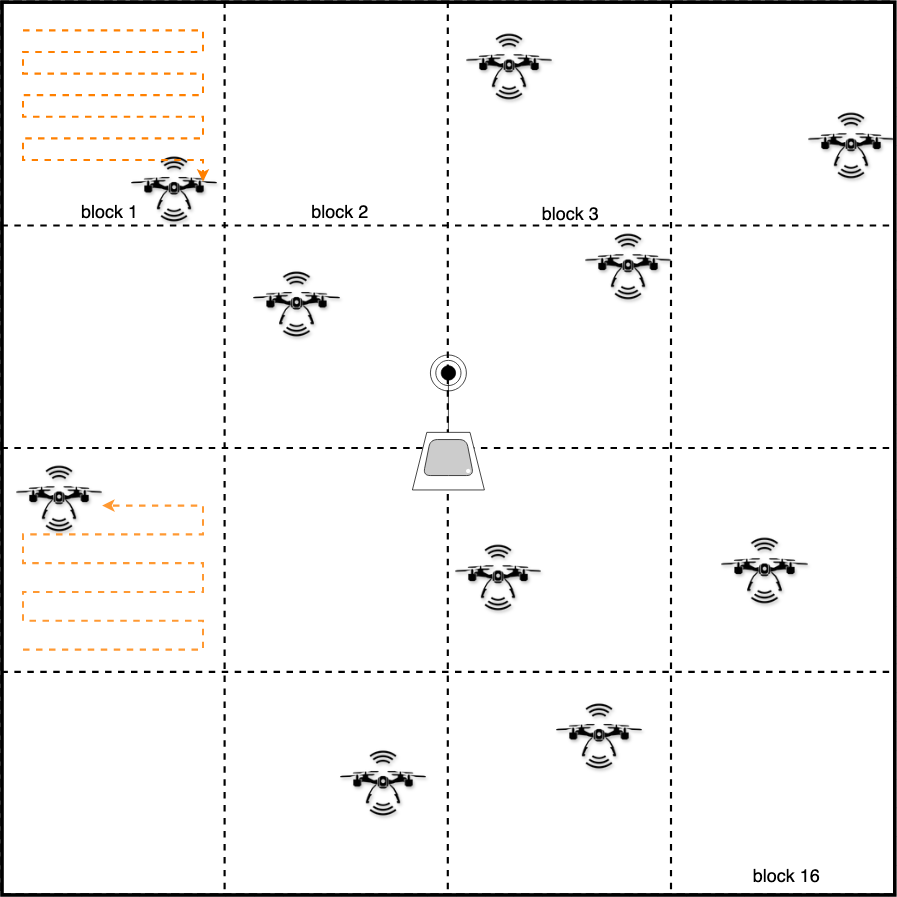
\includegraphics[height = 8 cm]{image/DroniInArea.png}%
    \ 
    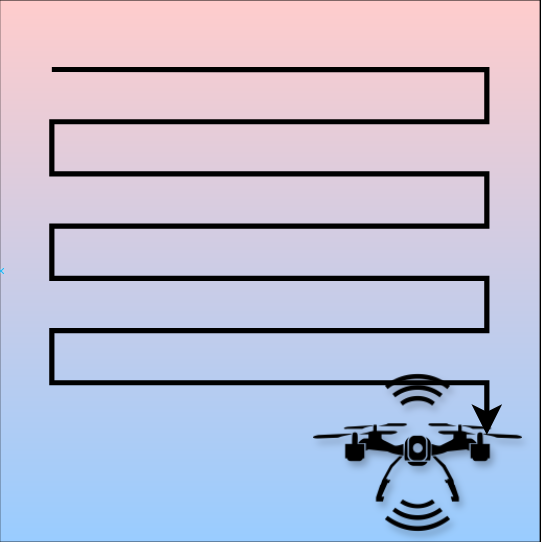
\includegraphics[height = 4 cm]{image/DroneInBlock.png}
    \caption{Esempio di area suddivisa in blocchi. Nel dettaglio a destra oltre al percorso seguito dal drone, viene evidenziata come più "calda" l'area visitata da meno tempo e più "fredda" l'area appena vista.}
\end{figure}

\begin{figure}[H]
    \centering
    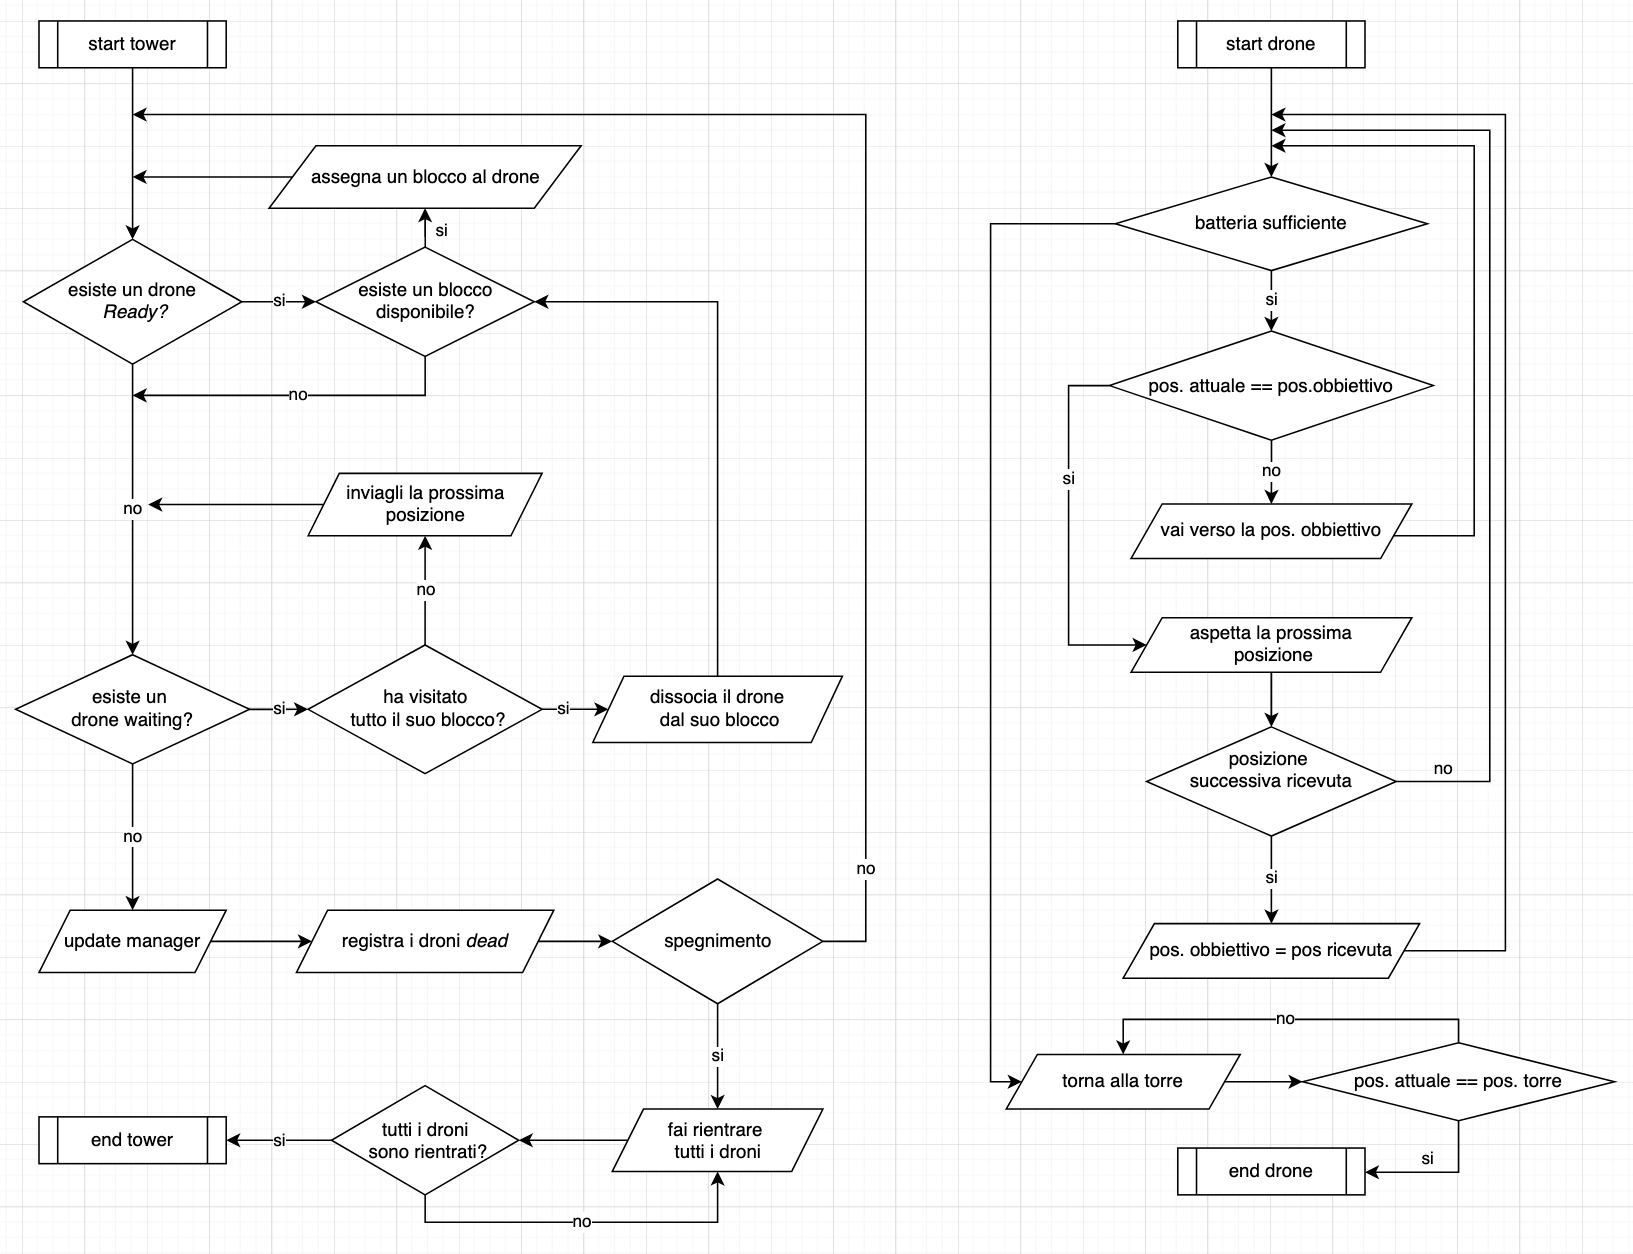
\includegraphics[height = 16 cm]{image/FlowCharts.png}
    \caption{FlowChart della torre e del drone. Nota bene, nel FlowChart viene assunto che il drone e la torre siano già connessi}
    
\end{figure}

\begin{figure}[H]
    \centering
    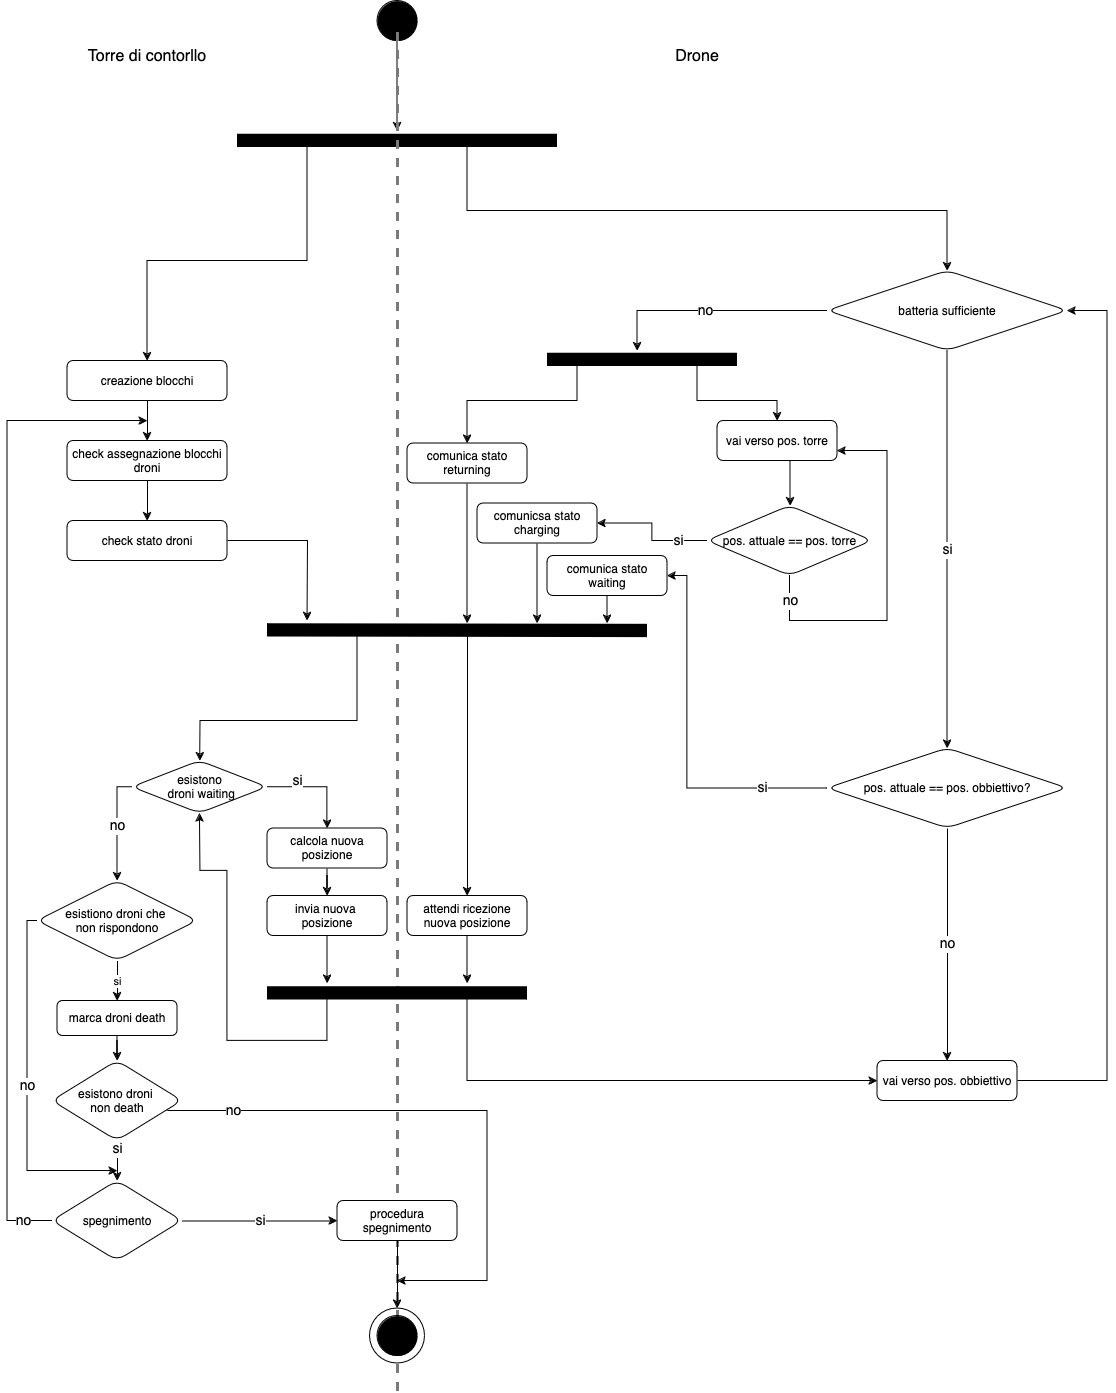
\includegraphics[height = 17 cm]{image/activitiDiagram.png}
    \caption{Activity diagram del sistema di interazione e decisione tra torre e drone, nel diagramma sono mostrate due barriere in cui drone e torre si sincronizzano per scambiarsi i messaggi principali mentre è lasciato implicito l'handler message di entrambi per messaggi di check.}
    
\end{figure}


\newpage
\subsubsection{State diagram}
Per decidere l'azione da assegnare ad ogni drone la torre deve riuscire a distinguere la condizione di ogni drone. 
Definiamo quindi $6$ stati in cui ogni drone può trovarsi:
\begin{enumerate}
    \item \textbf{CHARGING:} il drone si trova alla base, e sta ricaricando la sua batteria
    \item \textbf{READY:} il drone è carico e si trova nella torre di controllo (è pronto a partire)
    \item \textbf{WAITING:} il drone sta aspettando che la torre gli invii la prossima coordinata
    \item \textbf{MONITORING:} il drone sta scansionando l'area che gli è stata assegnata seguendo i punti inviati dalla torre
    \item \textbf{RETURNING:} la carica del drone è sufficiente solo per il suo rientro (il drone sta rientrando)
    \item \textbf{DEAD:} la batteria del drone si è scaricata prima che questo potesse rientrare oppure la torre di controllo non riesce più a contattarlo (fault).
\end{enumerate}
\begin{figure}[h]
    \centering
    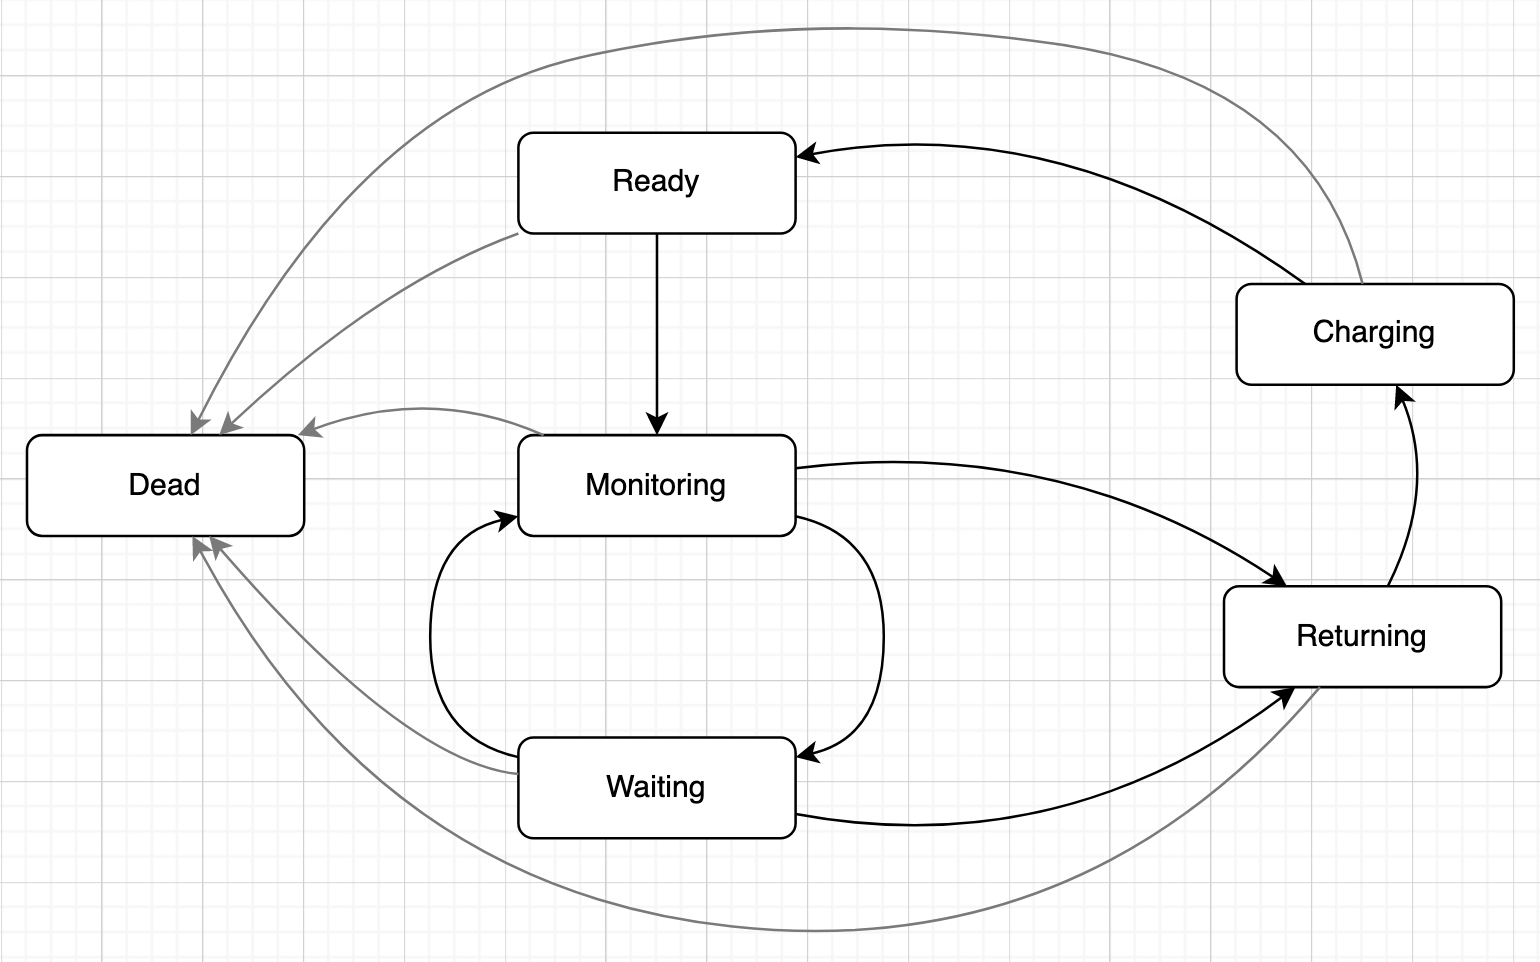
\includegraphics[height = 8 cm]{image/StateDiagram.png}
    \caption{State diagram}
\end{figure}
\subsubsection{Scelte progettuali}
\paragraph*{Divisione dei blocchi}
Dato che un punto si considera visitato se si trova nel raggio di 10 metri da un drone, possiamo discretizzare l'area rappresentandola come una matrice di case quadrate di dimensione $10\sqrt{2} \times 10\sqrt{2}$
\begin{figure}[h]
    \centering
    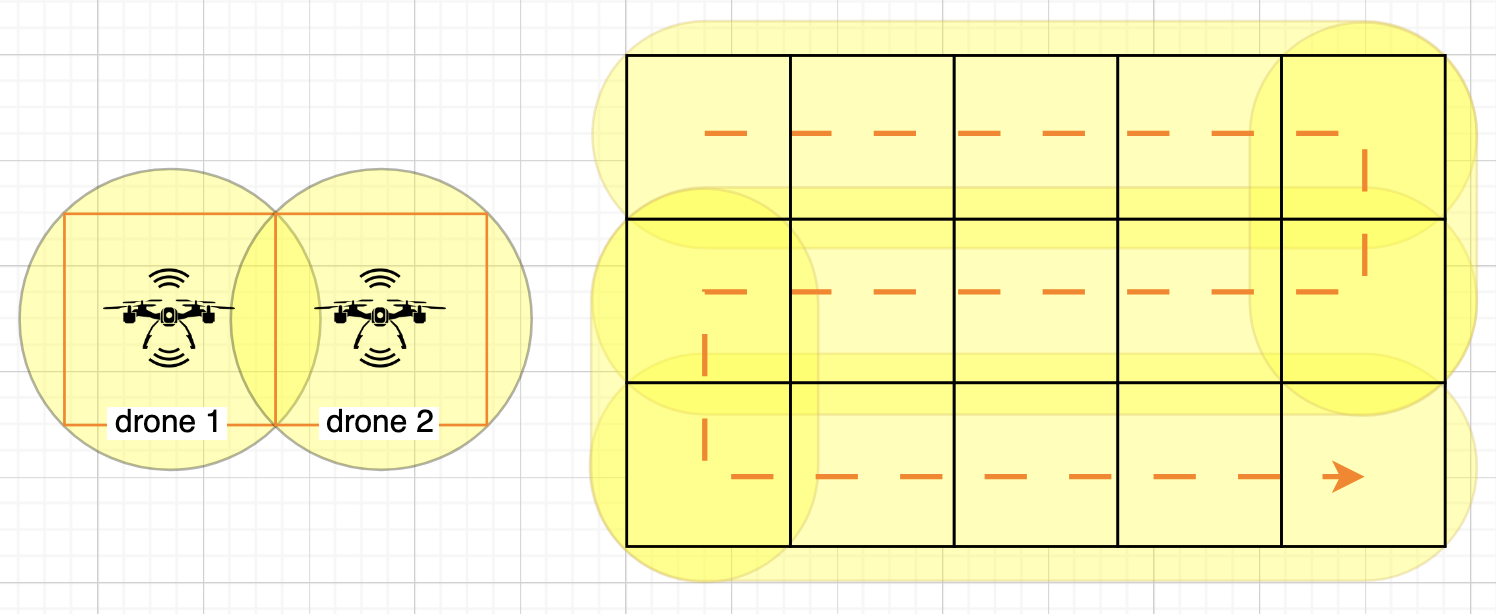
\includegraphics[height = 5 cm]{image/areedroni.png}
    \caption{L'area divisa in caselle della dimensione del quadrato inscritto nel cerchio di raggio 10}
\end{figure}

Abbiamo scelto di raggruppare le caselle in blocchi tutti uguale area per garantire equità nelle assegnazioni. 
Data la variabilità delle dimensioni dell'area e del numero di droni in fase iniziale, non è sempre garantito che il numero di droni divida il numero caselle in un valore utile per costruire una matrice di blocchi, utilizziamo un valore di blocchi maggiore per garantirne la perfetta di visibilità in sottoaree uguali.
Questo permette a tutti i droni \textit{READY} di volare contemporaneamente all'inizio del processo di monitoraggio e quindi ridurre il più possibile il tempo di visita medio dell'intera area.
Anche se creare più blocchi ne riduce le dimensioni, questo non influisce sulle prestazioni del sistema in quanto ogni drone quando termina il ciclo di visita del suo blocco inizia a visitarne un altro e continua finché la batteria lo permette.


\paragraph*{Assegnamento dei blocchi}
Per minimizzare il tempo di visita massimo e medio abbiamo sperimentato due criteri di scelta:
\begin{enumerate}
    \item \textbf{FirstAverageTime}: Assegnare ad un drone \textit{free} il blocco con tempo medio trascorso dall'ultima visita più alto (la media viene eseguita su tutte le caselle nel blocco).
    
    \item \textbf{FirstMaxTime}: Assegnare ad un drone \textit{free} il blocco che contiene la casella visitata meno di recente.
\end{enumerate}
Attualmente il programma utilizza il secondo approccio (\textbf{FirstMaxTime}). Se valutiamo il criterio di assegnamento basandoci su tempo di visita medio e tempo di visita massimo raggiunto durante una simulazione, 
possiamo osservare che a parità di area e di droni il FirstAverageTime ottiene un tempo di visita medio leggermente più basso di quello del FirstMaxTime ma un tempo massimo più alto in quanto tende a non riassegnare dei blocchi (magari quelli più ai margini) che hanno pochi punti con un tempo di visita molto alto ma molti con tempo di visita molto basso.
Al contrario il FirstMaxTime al costo di aumentare leggermente il tempo medio di visita, riesce a diminuire sensibilmente il tempo di visita massimo dimostrandosi più equo.  


\section{Protocollo di comunicazione}
La Torre di Controllo ed i Droni comunicano in maniera asincrona. Le comunicazioni avvengono tramite Redis.
\subsection{Scambio di messaggi}

Ogni attore ha un suo identificativo univoco. La torre ha sempre ID = 0 mentre i droni hanno id casuali assegnati dalla torre. 
Ogni attore ha riservato un canale rappresentato su redis da una \textbf{coda} con chiave = "c:\textbf{id}"

Il proprietario usa il suo canale solo in lettura mentre gli altri attori lo utilizzano in scrittura.
Dunque ogni elemento nella coda rappresenta l'id di un messaggio con il seguente formato $(m:ID:mID)$ dove
\begin{itemize}
    \item $ID$ rappresenta l'id del mittente
    \item $mID$ rappresenta l'identificatore univoco dell'elemento nel canale.
\end{itemize}

Il contenuto del messaggio si ottiene inserendo in un apposito \textbf{HashMap} l'$mID$ del messaggio.
\subsection{La classe Channel}
Per gestire agevolmente la ricezione e l'invio dei messaggio è stata implementata la classe Channel, la quale gestisce un canale di un attore. Per inviare e ricevere messaggi, la classe channel presenta due metodi:
I messaggi vengono letti e scritti dalla coda utilizzando \textbf{"LPUSH c:id message\_id"} per inserire un messaggio, ed \textbf{"RPOP c:id"} per estrarre il primo messaggio arrivato.

\textbf{void sendMessageTo(int channelId, Message \&message)}\\
Questo metodo permette di aggiungere alla lista di messaggi di channelId il messaggio message tramite i due comandi:

\begin{lstlisting}[style=customcpp, caption={da tower.cpp}]
    // Creazione del messaggio su redis
    hset m:{this.id}:{message.id} {message.parseMessage()}
    
    // Aggiunta del messaggio al canale
    lpush c:{channelId} m:{this.id}:{message.id} 
\end{lstlisting}

\textbf{Message* awaitMessage(long timeout = -1)}\\
Questo metodo serve per aspettare l'arrivo di un messaggio all'interno di un canale, per poi leggerlo e ritornarlo.
Il parametro \textbf{timeout}, se diverso da -1, imposta un tempo massimo per l'attesa di un messaggio.
\subsubsection{Thread Safety}

La Classe channel è thread safe, poiché gestisce le due funzioni \textbf{sendMessageTo} e \textbf{awaitMessage} tramite due mutex:
\begin{itemize}
    \item Un mutex in scrittura, che viene utilizzato per fare il lock durante la creazione e scrittura di un messaggio su un canale
    \item Un mutex in lettura, che viene lockato in attesa di una risposta da redis quando si tenta di leggere un messaggio dal canale.
\end{itemize}

Si è deciso di dividere le operazioni tra due mutex per questione di efficienza, così che mentre un attore è in attesa di un messaggio,
possa continuare a fare altre operazioni in scrittura per aggiornare il suo stato agli occhi degli altri attori (nel nostro caso, 
torna utile per ridurre i tempi di attesa di risposta tra la torre ed i droni)
\subsection{La classe Message}
La classe Message è la classe che rappresenta un messaggio di un canale.
\subsubsection{Costruttori}
I costruttori della classe Message sono due:
\begin{itemize}
    
    \item \textbf{Message(std::string id)}\\
        Usato nella creazione di un messaggio già presente.
        Prende come parametro una stringa del formato \textbf{id:mid}, nel quale \textbf{id} è l'id del canale che ha inviato il messaggio, e \textbf{mid} è l'id del messaggio.

    \item \textbf{Message(int id)}\\
        Usato nella creazione di un messaggio da creare ed inviare.
        Prende come parametro un intero che rappresenta l'id del messaggio.

\end{itemize}
In aggiunta, questa classe presenta due metodi virtuali che deve implementare ogni tipo di messaggio:\\
\begin{itemize}
    \item \textbf{void parseResponse(RedisResponse* response)}\\
        Questo metodo serve a ricevere una Risposta da un Comando Redis, e tramutarla in messaggio. Dietro le quinte, quello che viene fatto è:
        \begin{enumerate}
            \item Inviare un comando a redis del tipo \textit{hgetall n:id:mid}
            \item Controllare la validità della risposta
            \item Creare un messaggio tramite il costruttore:\\ \textit{Message(std::string id)}
            \item Parsare la risposta ottenuta tramite: \\ \textit{message.parseResponse(response)}
        \end{enumerate}
    \item\textbf{std::string parseMessage()}\\
        Questo metodo serve a trasformare i dati contenuti nel messaggio in una stringa della forma:
        \begin{verbatim}
            type type_value p1 v1 p2 v2 p3 v3
        \end{verbatim}
        Nella quale type\_value è un intero che rappresenta il tipo del messaggio, mentre pX kX sono le coppie (parametro, valore) contenute nel messaggio

\end{itemize}



\textbf{Esempio:} La classe PositionMessage, che serve per mandare la posizione di un drone alla torre, presenterà il corpo della funzione parseMessage() di questo tipo:
\begin{lstlisting}[style=customcpp, caption={da tower.cpp}]
    return "type 2 x " + std::to_string(this->x) + " y " + std::to_string(this->y);
\end{lstlisting}
\subsubsection{Lista Messaggi}

% Definisce una nuova colonna di tipo "L" che è equivalente alla "l" ma più versatile per l'ambiente tabularx
\newcolumntype{L}{>{\raggedright\arraybackslash}X}

% Ridurre la dimensione del carattere della tabella
\small

\begin{adjustbox}{max width=\textwidth}
    \begin{tabularx}{\textwidth}{|L|c|L|L|}
    \hline
    \rule{0pt}{3ex} % Aggiungi spazio verticale
    \textbf{Classe} & \textbf{Tipo} & \textbf{Parametri} & \textbf{Info} \\
    \hline
    \rule{0pt}{3ex} % Aggiungi spazio verticale
    AssociateMessage & 0 & drone\_id: long long, x: int, y: int & Messaggio di associazione drone$\leftrightarrow$torre \\
    \hline
    \rule{0pt}{3ex} % Aggiungi spazio verticale
    PingMessage & 1 & nessuno & Semplice messaggio di Ping \\
    \hline
    \rule{0pt}{3ex} % Aggiungi spazio verticale
    DroneInfoMessage & 2 & {params} & Scambio parametri drone$\rightarrow$torre \\
    \hline
    \rule{0pt}{3ex} % Aggiungi spazio verticale
    LocationMessage & 3 & x: int, y: int & Nuova posizione per drone dalla torre \\
    \hline
    \rule{0pt}{3ex} % Aggiungi spazio verticale
    RetireMessage & 4 & nessuno & Drone con batteria scarica. Rientro necessario \\
    \hline
    \rule{0pt}{3ex} % Aggiungi spazio verticale
    DisconnectMessage & 5 & nessuno & Disconnette l'associazione drone$\leftrightarrow$torre \\
    \hline
    \end{tabularx}
\end{adjustbox}

\textbf{AssociateMessage}

\begin{myindentpar}{0.4cm}
Messaggio inviato dal drone alla torre per richiedere l'associazione al pool di droni.
La torre risponde ritornando l'id che associerà al drone per riconoscimento all'interno della formazione.
Il messaggio presenta il campo \textbf{drone\_id}, che rappresenta l'id temporaneo de drone in richiesta, oppure l'id associato dalla torre in caso di associazione effettuata.
Inoltre, il messaggio contiene la posizione della torre per gestire con precisione il punto di partenza dei droni.
\end{myindentpar}

\textbf{PingMessage}
\begin{myindentpar}{0.4cm}
Messaggio inviato dalla torre al drone per verificarne l'esistenza. Viene generalmente utilizzato quando la torre non riceve update dal drone per più di 2 minuti.
Questo messaggio non presenta parametri.
\end{myindentpar}

\textbf{DroneInfoMessage}
\begin{myindentpar}{0.4cm}
Messaggio per aggiornare le info di un drone all'interno del db della torre. Viene generalmente mandato dalla torre al drone, per richiedere un update dello stato del drone e verificarne il funzionamento.
I parametri del messaggio sono i campi del drone:
\begin{itemize}
    \item drone\_id
    \item x
    \item y
    \item drone\_state
    \item charge\_time
    \item battery\_autonomy
\end{itemize}
\end{myindentpar}

\textbf{LocationMessage}
\begin{myindentpar}{0.4cm}
Messaggio con duplice scopo:
\begin{itemize}
    \item Se inviato dalla torre al drone, significa che la torre sta impostando delle nuove coordinate da raggiungere al drone. Dunque, in lettura il drone aggiornerà le coordinate e deciderà cosa fare di conseguenza.
    \item Se inviato dal drone alla torre, rappresenta un update della posizione del drone, il quale ha completato il movimento assegnatogli in precedenza.
\end{itemize}
Il messaggio presenta i seguenti parametri:
\begin{itemize}
    \item x: La posizione sull'asse x
    \item y: La posizione sull'asse y
\end{itemize}
\end{myindentpar}

\textbf{RetireMessage}
\begin{myindentpar}{0.4cm}
Messaggio inviato dal drone per notificare la necessità di rientro per low battery.
In questo caso, la torre invia al drone un LocationMessage con le coordinate precise della torre, e lo mette in stato retiring per ottimizzare il percorso di rientro.
\end{myindentpar}

\textbf{DisconnectMessage}
\begin{myindentpar}{0.4cm}
Messaggio che rimuove l'associazione tra la torre ed il drone. Permette di liberare risorse su redis e sul database.
\end{myindentpar}
\newpage

\subsection{Message Sequence Chart UML}
Di seguito vengono mostrati alcuni \textbf{Message Sequence Chart UML} che mostrano i principali scenari di scambio di messaggi tra la torre e un drone qualsiasi.



\begin{tabular}{m{0.5 \textwidth} p{0.5 \textwidth}}
    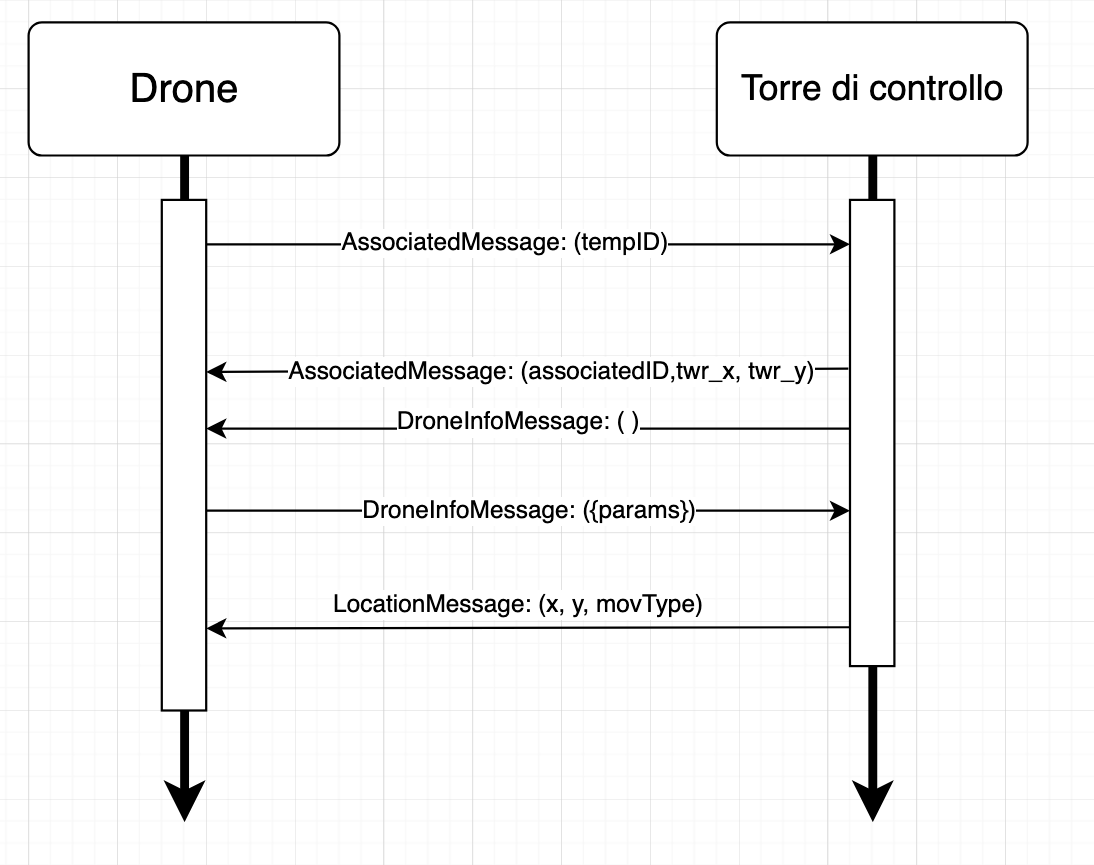
\includegraphics[width=0.45\textwidth]{image/associatedUML_MSC.png}&\textbf{Associazione di un drone:}
    \begin{enumerate}
        \item Il drone richiede di essere associato 
        \item La torre aderisce all'associazione
        \item La torre richiede le informazioni del drone
        \item Il drone risponde alla richiesta di informazioni 
        \item La torre inizia a guidare il drone 
    \end{enumerate}\\
    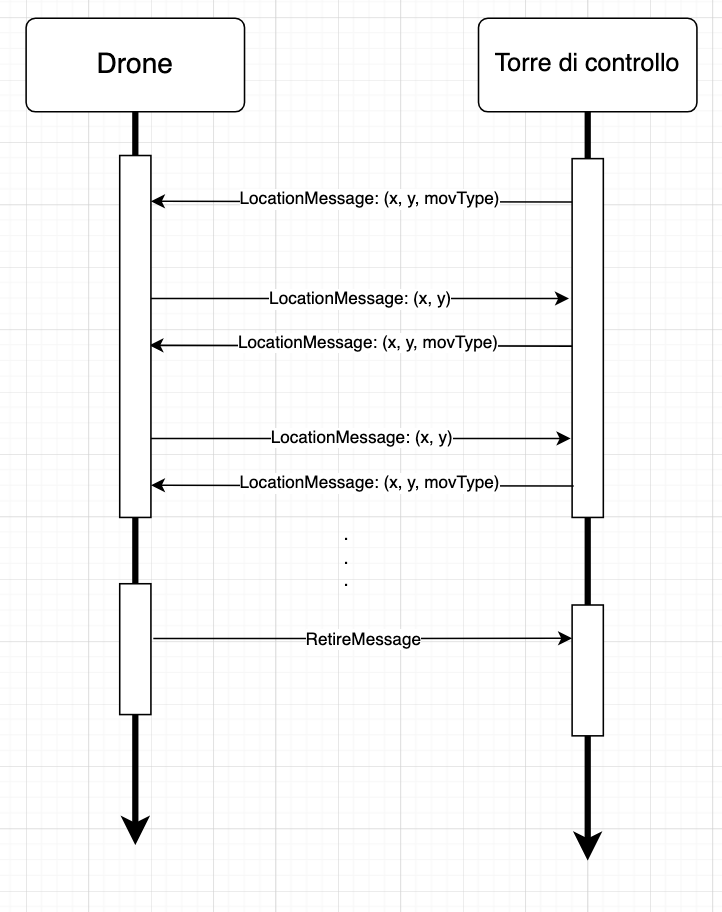
\includegraphics[width=0.45\textwidth]{image/monitoringUML_MSC.png} &\textbf{Monitoraggio di un drone:}
    \begin{enumerate}
        \item La torre invia la posizione da raggiungere
        \item Tramite il \textit{LocationMessage} il drone comunica di aver raggiunto il punto identificato
        \item La torre prontamente risponde con il nuovo punto calcolato
        \item Quando il drone non ha carica sufficiente invia un \textit{RetireMessage} e torna alla torre
    \end{enumerate}\\
    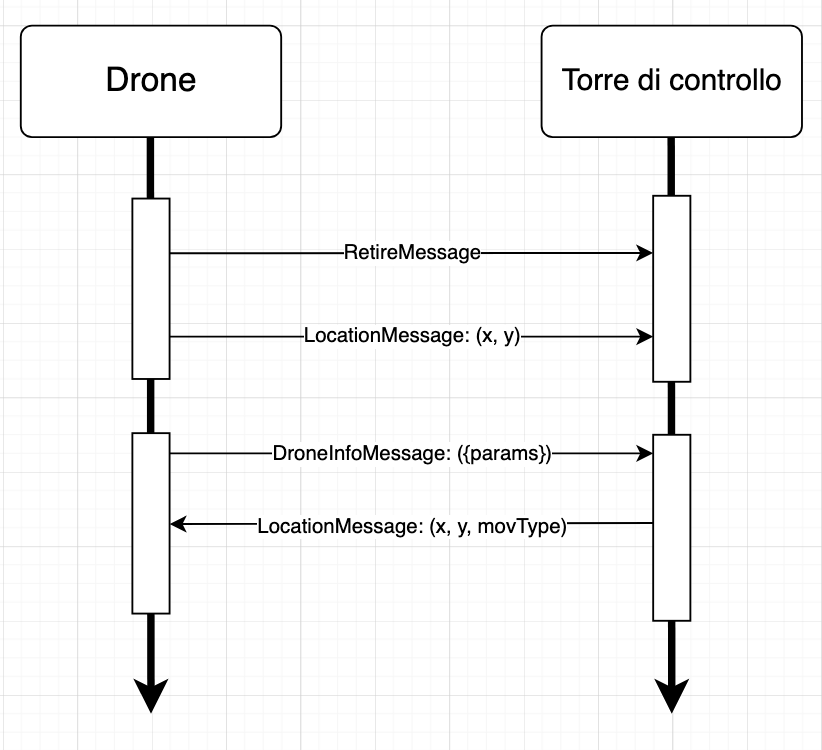
\includegraphics[width=0.45\textwidth]{image/rechargingUML_MSC.png}&\textbf{Ricarica di un drone:}
    \begin{enumerate}
        \item Il drone comunica che la sua batteria è scarica 
        \item Tramite il \textit{LocationMessage} il drone comunica di essere tornato alla torre 
        \item Il drone comunica di essersi ricaricato inviando un \textit{DroneInfoMessage}
        \item La torre ricomincia a guidarlo per monitorare l'area
    \end{enumerate}

\end{tabular}
\newpage
\section{Implementazione}
Di seguito vengono riportate parti del codice implementato 
\begin{lstlisting}[style=customcpp, caption={da drone.cpp}]
    void Drone::start(float executionSpeed) {

        this->setExecutionSpeed(executionSpeed);

        // Enstablish connection to tower
        bool connectedToTower = this->connectToTower();
        if (!connectedToTower) {
            loge("Can't connect to tower!");
            return;
        }
        logi("Connected to tower");

        // Start loop
        std::thread moveThread(&Drone::behaviourLoop, this);

        std::vector<std::thread> threads;
        this->running = true;
        this->setState(READY);
        while (this->running) {
            Message *message = this->channel->awaitMessage();
            if (message == nullptr) {
                // No message received. Maybe ping tower?
                continue;
            }
            logi("Received message m:" + message->getFormattedId());
            threads.emplace_back(&Drone::handleMessage, this, message);
            // Free up completed threads
            for (auto it = threads.begin(); it != threads.end();) {
                if (it->joinable()) {
                    it ++;
                } else {
                    it = threads.erase(it);
                }
            }
        }
        // Disconnect drone
        // Wait threads to finish
        for (auto &thread : threads) {
            thread.join();
        }

    }
    \end{lstlisting}
    Il drone dopo aver completato con successo la procedura di connessione, entra in un loop in cui gestisce parallelamente sia i suoi spostamenti [riga 14.  behaviourLoop è una funzione che simula lo spostamento del drone] sia i messaggi ricevuti e da inviare alla torre di controllo.
    \newpage
    Le funzioni utilizzate per suddividere l'area in blocchi
    \begin{lstlisting}[style=customcpp, caption={da area.cpp}]

    void calculateBlocksInArea(int width, int height, int &numBlocks, int &blockWidth, int &blockHeight) {
        int w = std::sqrt(numBlocks);
        int h = w;
        while (h * w < numBlocks) {
            if ((h + 1) * w <= numBlocks) {
                h++;
            } else {
                w++;
            }
        }
        numBlocks = w * h;
        blockWidth = std::ceil(static_cast<double>(width) / w);
        blockHeight = std::ceil(static_cast<double>(height) / h);
    }

    void Area::initArea(int blockCount, int centerX, int centerY) {
        this->blocks = new std::vector<Block>();
        int blockWidth = 0;
        int blockHeight = 0;
        calculateBlocksInArea(this->width, this->height, blockCount, blockWidth, blockHeight);
        logDebug("Area", "Area Approximated to " + std::to_string(blockCount) + "(" + std::to_string(blockWidth) + "," + std::to_string(blockHeight) + ")");
        int x = 0;
        int y = 0;
        for (int i = 0; i < blockCount; i++) {
            Block b(x, y, blockWidth, blockHeight);
            x += blockWidth;
            if (b.getX() >= this->width) {
                b.setX(0);
                b.setY(b.getY() + blockHeight);
                x = blockWidth;
                y += blockHeight;
            }
            if (b.getY() >= this->height) {
                // Extra blocks
                break;
            }
            if (b.getX() + b.getWidth() >= this->width) {
                b.setWidth(this->width - b.getX());
            }
            if (b.getY() + b.getHeight() >= this->height) {
                b.setHeight(this->height - b.getY());
            }
            b.orientBlock(centerX, centerY);
            this->blocks->push_back(b);
        }
        logDebug("Area", "Fitted " + std::to_string(this->blocks->size()) + " blocks");
    }
\end{lstlisting}
\newpage
La funzione che gestisce il principale comportamento della torre
\begin{lstlisting}[style=customcpp, caption={da tower.cpp}]
    void Tower::start() {
        if (!this->channel->isUp()) {
            loge("Can't start tower without a connected channel!");
            return;
        }
        // Register signals
        signal(SIGINT, Tower::handleSignal);
        signal(SIGTERM, Tower::handleSignal);
        this->running = true;
        std::vector<std::thread> threads;
        threads.emplace_back(&Tower::droneCheckLoop, this);
        // threads.emplace_back(&Tower::areaUpdateLoop, this);
        threads.emplace_back(&Tower::drawGrid, this);
        logi("Tower online");
        while (this->running) {
            // 1' of waiting before restarting the cycle
            Message *message = this->channel->awaitMessage(10);
            if (message == nullptr) {
                // If we have no message to handle, we check last updates from drones
                // If a last update is > x second (to decide, maybe 1-5' => 60-300'') -> ping and wait a response
                // If the drone is doing nothing, we commit it to monitor a zone
            } else {
                // Handle message received on another thread, and return to listen
                logi("Received message from Drone " + std::to_string(message->getChannelId()) + ". Type: " + std::to_string(message->getType()));
                threads.emplace_back(&Tower::handleMessage, this, message);
            }
            // Free finished threads
            for (auto it = threads.begin(); it != threads.end(); ) {
                if (it->joinable()) {
                    it++;
                } else {it = threads.erase(it);}
            }
        }
        logi("Powering Off");
        // Disconnect Drones
        std::vector<Drone> drones = this->getDrones();
        for (Drone& drone : drones) {
            if (drone.droneState == DEAD) {
                continue;
            }
            DisconnectMessage *message = new DisconnectMessage(this->generateMessageId());
            this->channel->sendMessageTo(drone.id, message);
            delete message;
        }
        logi("Waiting threads to finish");
        // Await Spawned Threads
        for (auto& thread : threads) {
            thread.join();
        }
        // Flush Channel
        logi("Flushing Channel");
        bool channelFlushed = this->channel->flush();
        if (channelFlushed) {
            logi("Channel Flushed!");
        } else {
            logw("Can't flush redis channel");
        }
        logi("Printing Area");
        std::ofstream areaFile;
        areaFile.open("area.csv", std::ios_base::app);
        for(int i = 0; i < this->areaWidth; i++) {
            for(int j = 0; j < this->areaHeight; j++) {
                areaFile << this->area->operator[](i)[j] << ",";
            }
            areaFile << "\n";
        }
        areaFile.close();
        logi("Area Saved on area.scv");
    }

\end{lstlisting}
La funzione che la torre di controllo utilizza per decidere la prossima posizione da inviare ad un particolare drone
\begin{lstlisting}[style=customcpp, caption={da tower.cpp}]
    void Tower::calcolateDronePath(Drone drone) {
        // Check Active Block
        std::vector<Block> *blocks = this->area->getBlocks();
        for (Block& block : *blocks) {
            if (block.getAssignment() == drone.id) {
                // Check block cells
                if (block.getLastX() != drone.posX || block.getLastY() != drone.posY) {
                    block.setLastX(drone.posX);
                    block.setLastY(drone.posY);
                }
                int x = block.getLastX() + block.getDirX();
                int y = block.getLastY();
                if (x == this->x && y == this->y) {
                    logi("Skipping Tower Cell");
                    // Safe because the tower is in the middle
                    x += block.getDirX();
                }
                if (x >= block.getX() + block.getWidth() || x < block.getX()) {
                    y += block.getDirY();
                    x -= block.getDirX();
                    if (y > block.getY() + block.getHeight() || y < block.getY()) {
                        // Reset Block and Associate a new One
                        this->associateBlock(drone);
                        block.reset(this->x, this->y);
                        return;
                    }
                    block.setDirX(-block.getDirX());
                }
                LocationMessage *location = new LocationMessage(generateMessageId());
                location->setLocation(x, y);
                this->channel->sendMessageTo(drone.id, location);
                delete location; 
                return;
            }
        }
        // Not Returned before -> no Block associated
        this->associateBlock(drone);
    }
\end{lstlisting}

\end{document}

